\documentclass[twoside]{book}

% Packages required by doxygen
\usepackage{fixltx2e}
\usepackage{calc}
\usepackage{doxygen}
\usepackage[export]{adjustbox} % also loads graphicx
\usepackage{graphicx}
\usepackage[utf8]{inputenc}
\usepackage{makeidx}
\usepackage{multicol}
\usepackage{multirow}
\PassOptionsToPackage{warn}{textcomp}
\usepackage{textcomp}
\usepackage[nointegrals]{wasysym}
\usepackage[table]{xcolor}

% Font selection
\usepackage[T1]{fontenc}
\usepackage[scaled=.90]{helvet}
\usepackage{courier}
\usepackage{amssymb}
\usepackage{sectsty}
\renewcommand{\familydefault}{\sfdefault}
\allsectionsfont{%
  \fontseries{bc}\selectfont%
  \color{darkgray}%
}
\renewcommand{\DoxyLabelFont}{%
  \fontseries{bc}\selectfont%
  \color{darkgray}%
}
\newcommand{\+}{\discretionary{\mbox{\scriptsize$\hookleftarrow$}}{}{}}

% Page & text layout
\usepackage{geometry}
\geometry{%
  a4paper,%
  top=2.5cm,%
  bottom=2.5cm,%
  left=2.5cm,%
  right=2.5cm%
}
\tolerance=750
\hfuzz=15pt
\hbadness=750
\setlength{\emergencystretch}{15pt}
\setlength{\parindent}{0cm}
\setlength{\parskip}{3ex plus 2ex minus 2ex}
\makeatletter
\renewcommand{\paragraph}{%
  \@startsection{paragraph}{4}{0ex}{-1.0ex}{1.0ex}{%
    \normalfont\normalsize\bfseries\SS@parafont%
  }%
}
\renewcommand{\subparagraph}{%
  \@startsection{subparagraph}{5}{0ex}{-1.0ex}{1.0ex}{%
    \normalfont\normalsize\bfseries\SS@subparafont%
  }%
}
\makeatother

% Headers & footers
\usepackage{fancyhdr}
\pagestyle{fancyplain}
\fancyhead[LE]{\fancyplain{}{\bfseries\thepage}}
\fancyhead[CE]{\fancyplain{}{}}
\fancyhead[RE]{\fancyplain{}{\bfseries\leftmark}}
\fancyhead[LO]{\fancyplain{}{\bfseries\rightmark}}
\fancyhead[CO]{\fancyplain{}{}}
\fancyhead[RO]{\fancyplain{}{\bfseries\thepage}}
\fancyfoot[LE]{\fancyplain{}{}}
\fancyfoot[CE]{\fancyplain{}{}}
\fancyfoot[RE]{\fancyplain{}{\bfseries\scriptsize 制作者 Doxygen }}
\fancyfoot[LO]{\fancyplain{}{\bfseries\scriptsize 制作者 Doxygen }}
\fancyfoot[CO]{\fancyplain{}{}}
\fancyfoot[RO]{\fancyplain{}{}}
\renewcommand{\footrulewidth}{0.4pt}
\renewcommand{\chaptermark}[1]{%
  \markboth{#1}{}%
}
\renewcommand{\sectionmark}[1]{%
  \markright{\thesection\ #1}%
}

% Indices & bibliography
\usepackage{natbib}
\usepackage[titles]{tocloft}
\setcounter{tocdepth}{3}
\setcounter{secnumdepth}{5}
\makeindex

% Hyperlinks (required, but should be loaded last)
\usepackage{ifpdf}
\ifpdf
  \usepackage[pdftex,pagebackref=true]{hyperref}
\else
  \usepackage[ps2pdf,pagebackref=true]{hyperref}
\fi
\hypersetup{%
  colorlinks=true,%
  linkcolor=blue,%
  citecolor=blue,%
  unicode%
}

% Custom commands
\newcommand{\clearemptydoublepage}{%
  \newpage{\pagestyle{empty}\cleardoublepage}%
}

\usepackage{caption}
\captionsetup{labelsep=space,justification=centering,font={bf},singlelinecheck=off,skip=4pt,position=top}

%===== C O N T E N T S =====

\begin{document}

% Titlepage & ToC
\hypersetup{pageanchor=false,
             bookmarksnumbered=true,
             pdfencoding=unicode
            }
\pagenumbering{alph}
\begin{titlepage}
\vspace*{7cm}
\begin{center}%
{\Large C\+C\+\_\+\+P\+U\+S\+H\+\_\+\+S\+DK }\\
\vspace*{1cm}
{\large 制作者 Doxygen 1.8.13}\\
\end{center}
\end{titlepage}
\clearemptydoublepage
\pagenumbering{roman}
\tableofcontents
\clearemptydoublepage
\pagenumbering{arabic}
\hypersetup{pageanchor=true}

%--- Begin generated contents ---
\chapter{继承关系索引}
\section{类继承关系}
此继承关系列表按字典顺序粗略的排序\+: \begin{DoxyCompactList}
\item N\+S\+Object\begin{DoxyCompactList}
\item \contentsline{section}{Offline\+Play\+Back}{\pageref{interface_offline_play_back}}{}
\item \contentsline{section}{Play\+Parameter}{\pageref{interface_play_parameter}}{}
\item \contentsline{section}{Request\+Data}{\pageref{interface_request_data}}{}
\item \contentsline{section}{Request\+Data\+Play\+Back}{\pageref{interface_request_data_play_back}}{}
\item \contentsline{section}{Save\+Log\+Util}{\pageref{interface_save_log_util}}{}
\end{DoxyCompactList}
\item $<$N\+S\+Object$>$\begin{DoxyCompactList}
\item \contentsline{section}{$<$Offline\+Play\+Back\+Delegate $>$}{\pageref{protocol_offline_play_back_delegate_01-p}}{}
\item \contentsline{section}{$<$Request\+Data\+Delegate $>$}{\pageref{protocol_request_data_delegate_01-p}}{}
\item \contentsline{section}{$<$Request\+Data\+Play\+Back\+Delegate $>$}{\pageref{protocol_request_data_play_back_delegate_01-p}}{}
\end{DoxyCompactList}
\end{DoxyCompactList}

\chapter{类索引}
\section{类列表}
这里列出了所有类、结构、联合以及接口定义等,并附带简要说明\+:\begin{DoxyCompactList}
\item\contentsline{section}{\hyperlink{interface_offline_play_back}{Offline\+Play\+Back} }{\pageref{interface_offline_play_back}}{}
\item\contentsline{section}{\hyperlink{protocol_offline_play_back_delegate_01-p}{$<$\+Offline\+Play\+Back\+Delegate $>$} }{\pageref{protocol_offline_play_back_delegate_01-p}}{}
\item\contentsline{section}{\hyperlink{interface_play_parameter}{Play\+Parameter} }{\pageref{interface_play_parameter}}{}
\item\contentsline{section}{\hyperlink{interface_request_data}{Request\+Data} }{\pageref{interface_request_data}}{}
\item\contentsline{section}{\hyperlink{protocol_request_data_delegate_01-p}{$<$\+Request\+Data\+Delegate $>$} }{\pageref{protocol_request_data_delegate_01-p}}{}
\item\contentsline{section}{\hyperlink{interface_request_data_play_back}{Request\+Data\+Play\+Back} }{\pageref{interface_request_data_play_back}}{}
\item\contentsline{section}{\hyperlink{protocol_request_data_play_back_delegate_01-p}{$<$\+Request\+Data\+Play\+Back\+Delegate $>$} }{\pageref{protocol_request_data_play_back_delegate_01-p}}{}
\item\contentsline{section}{\hyperlink{interface_save_log_util}{Save\+Log\+Util} }{\pageref{interface_save_log_util}}{}
\end{DoxyCompactList}

\chapter{类说明}
\hypertarget{interface_c_c_push_util}{}\section{C\+C\+Push\+Util类 参考}
\label{interface_c_c_push_util}\index{C\+C\+Push\+Util@{C\+C\+Push\+Util}}
类 C\+C\+Push\+Util 继承关系图\+:\begin{figure}[H]
\begin{center}
\leavevmode
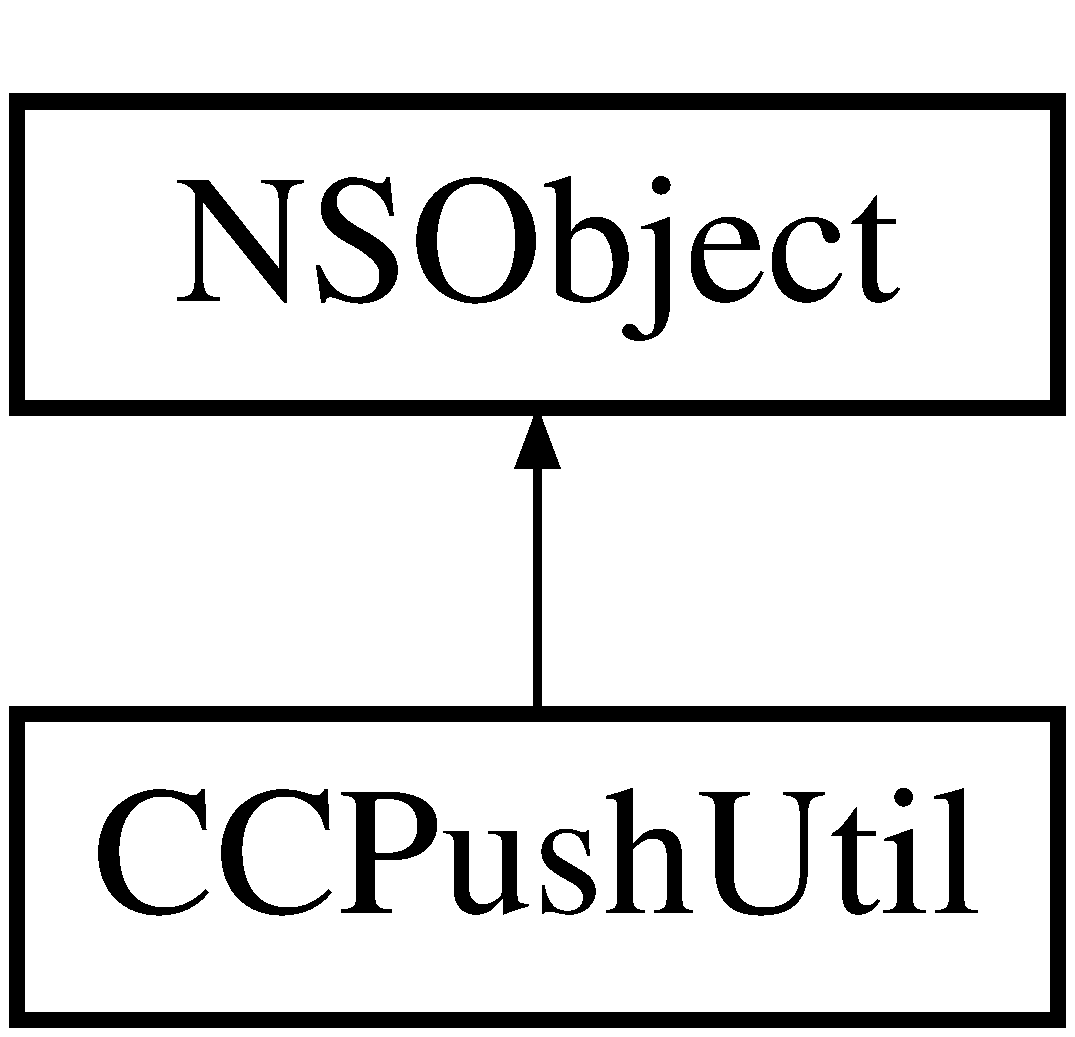
\includegraphics[height=2.000000cm]{interface_c_c_push_util}
\end{center}
\end{figure}
\subsection*{构造函数}
\begin{DoxyCompactItemize}
\item 
\mbox{\Hypertarget{interface_c_c_push_util_af81678969b596bc2e6c3e59415fde2aa}\label{interface_c_c_push_util_af81678969b596bc2e6c3e59415fde2aa}} 
(N\+S\+Integer) -\/ \hyperlink{interface_c_c_push_util_af81678969b596bc2e6c3e59415fde2aa}{get\+Max\+Bitrate}
\begin{DoxyCompactList}\small\item\em 得到房间可用的最大码率,注:在登录接口后,才能取到 \end{DoxyCompactList}\item 
(void) -\/ \hyperlink{interface_c_c_push_util_aab53c1f3bb2cdd070681aa497e4f5bf7}{start\+Push\+With\+Camera\+Front\+:}
\begin{DoxyCompactList}\small\item\em 开始推流,注:设置好码率,分辨率,帧率,和预览页面后才可以开始推流 \end{DoxyCompactList}\item 
(void) -\/ \hyperlink{interface_c_c_push_util_ae4f1a2d7f38053c47273360091c5c4ad}{login\+With\+Parameters\+:}
\begin{DoxyCompactList}\small\item\em 服务器请求初始化 \end{DoxyCompactList}\item 
\mbox{\Hypertarget{interface_c_c_push_util_a1778a6c31ea2b6df39f25bdd0861450a}\label{interface_c_c_push_util_a1778a6c31ea2b6df39f25bdd0861450a}} 
(void) -\/ \hyperlink{interface_c_c_push_util_a1778a6c31ea2b6df39f25bdd0861450a}{set\+Video\+Size\+:\+Bit\+Rate\+:\+Frame\+Rate\+:}
\begin{DoxyCompactList}\small\item\em 设置分辨率video\+Size,(重要:分辨率长宽一定要设置为偶数,否则推出来的视频会有绿边)建议不要设置太离谱,码率i\+Bit\+Rate,100到本房间可用的最大码率之间设置, 如果小于100,码率会设置成最小值100,如果码率大于最大码率,码率会设置成最大值,帧率i\+Frame\+Rate建议设置20到30之间, 小于20或大于30会设置成默认值25 \end{DoxyCompactList}\item 
(void) -\/ \hyperlink{interface_c_c_push_util_a5d7d1fe16a235b70c8c3fe7561d565bc}{set\+Preview\+:}
\begin{DoxyCompactList}\small\item\em 设置预览页面 \end{DoxyCompactList}\item 
\mbox{\Hypertarget{interface_c_c_push_util_a41c09116f2e237058972f918765a8169}\label{interface_c_c_push_util_a41c09116f2e237058972f918765a8169}} 
(void) -\/ \hyperlink{interface_c_c_push_util_a41c09116f2e237058972f918765a8169}{stop\+Push}
\begin{DoxyCompactList}\small\item\em 停止推流 \end{DoxyCompactList}\item 
\mbox{\Hypertarget{interface_c_c_push_util_ac1f328287df6b258312cb139f3be33bc}\label{interface_c_c_push_util_ac1f328287df6b258312cb139f3be33bc}} 
(void) -\/ \hyperlink{interface_c_c_push_util_ac1f328287df6b258312cb139f3be33bc}{set\+Camera\+Front\+:}
\begin{DoxyCompactList}\small\item\em 设置前后置摄像头 \end{DoxyCompactList}\item 
\mbox{\Hypertarget{interface_c_c_push_util_a280f4ead06a96bb58f25da97c85b09ad}\label{interface_c_c_push_util_a280f4ead06a96bb58f25da97c85b09ad}} 
(void) -\/ \hyperlink{interface_c_c_push_util_a280f4ead06a96bb58f25da97c85b09ad}{set\+Torch\+:}
\begin{DoxyCompactList}\small\item\em 开启闪光灯 \end{DoxyCompactList}\item 
\mbox{\Hypertarget{interface_c_c_push_util_a4494d30312c5ad7264bd08ae95e77d51}\label{interface_c_c_push_util_a4494d30312c5ad7264bd08ae95e77d51}} 
(void) -\/ \hyperlink{interface_c_c_push_util_a4494d30312c5ad7264bd08ae95e77d51}{set\+Mic\+Gain\+:}
\begin{DoxyCompactList}\small\item\em 设置声音大小,0-\/10,0和10分别表示静音和最大音量 \end{DoxyCompactList}\item 
\mbox{\Hypertarget{interface_c_c_push_util_ae178e219ed6572e239ebb018981a8607}\label{interface_c_c_push_util_ae178e219ed6572e239ebb018981a8607}} 
(void) -\/ \hyperlink{interface_c_c_push_util_ae178e219ed6572e239ebb018981a8607}{focux\+At\+Point\+:}
\begin{DoxyCompactList}\small\item\em 聚焦到某个点 \end{DoxyCompactList}\item 
(void) -\/ \hyperlink{interface_c_c_push_util_a1d24c1ff1a4f762e882a09650ec6fac4}{set\+Camera\+Beauty\+Filter\+With\+Smooth\+:white\+:pink\+:}
\begin{DoxyCompactList}\small\item\em 设置美颜滤镜 \end{DoxyCompactList}\item 
(void) -\/ \hyperlink{interface_c_c_push_util_ac6be9fb2ae7ecd8370ebe7f918aa4685}{add\+Water\+Mask\+:rect\+:}
\begin{DoxyCompactList}\small\item\em 设置水印(整个可设置的宽高和设置的屏幕分辨率,在切换摄像头之后需要在调用一次) \end{DoxyCompactList}\item 
(void) -\/ \hyperlink{interface_c_c_push_util_abeb3c0560246853b40729b3e091ef988}{publish\+Image\+:is\+Big\+:}
\begin{DoxyCompactList}\small\item\em 添加直播图片(添加图片到直播视频中,把图片直播出去) \end{DoxyCompactList}\item 
\mbox{\Hypertarget{interface_c_c_push_util_a1664d1e5d4b51a848f527a727430a422}\label{interface_c_c_push_util_a1664d1e5d4b51a848f527a727430a422}} 
(void) -\/ \hyperlink{interface_c_c_push_util_a1664d1e5d4b51a848f527a727430a422}{clear\+Publish\+Image}
\begin{DoxyCompactList}\small\item\em 清除直播图片 \end{DoxyCompactList}\item 
\mbox{\Hypertarget{interface_c_c_push_util_a91923b69cfb10c3dc40d247fdbb6fa45}\label{interface_c_c_push_util_a91923b69cfb10c3dc40d247fdbb6fa45}} 
(void) -\/ \hyperlink{interface_c_c_push_util_a91923b69cfb10c3dc40d247fdbb6fa45}{logout}
\begin{DoxyCompactList}\small\item\em 退出登录 \end{DoxyCompactList}\item 
(void) -\/ \hyperlink{interface_c_c_push_util_a5c4bc7eedd825fb399b1c0e77a3b7878}{set\+Node\+Index\+:}
\begin{DoxyCompactList}\small\item\em 设置推流节点索引,如果不设置,默认首选测速最优点(如果测速结果全部超时则会选择随机点) \end{DoxyCompactList}\item 
\mbox{\Hypertarget{interface_c_c_push_util_af7ad905ef9bfe2cee2631f9ca3343559}\label{interface_c_c_push_util_af7ad905ef9bfe2cee2631f9ca3343559}} 
(void) -\/ \hyperlink{interface_c_c_push_util_af7ad905ef9bfe2cee2631f9ca3343559}{test\+Speed}
\begin{DoxyCompactList}\small\item\em 测速 \end{DoxyCompactList}\item 
\mbox{\Hypertarget{interface_c_c_push_util_acd392a834f62338dd53eb5ad72be828a}\label{interface_c_c_push_util_acd392a834f62338dd53eb5ad72be828a}} 
(void) -\/ \hyperlink{interface_c_c_push_util_acd392a834f62338dd53eb5ad72be828a}{chat\+Message\+:}
\begin{DoxyCompactList}\small\item\em 发送公聊信息 \end{DoxyCompactList}\item 
\mbox{\Hypertarget{interface_c_c_push_util_af9f9ff382772ec3cf3b79494d54b98ef}\label{interface_c_c_push_util_af9f9ff382772ec3cf3b79494d54b98ef}} 
(void) -\/ \hyperlink{interface_c_c_push_util_af9f9ff382772ec3cf3b79494d54b98ef}{private\+Chat\+With\+Touserid\+:msg\+:}
\begin{DoxyCompactList}\small\item\em 发送私聊信息 \end{DoxyCompactList}\item 
\mbox{\Hypertarget{interface_c_c_push_util_a1cc7fcf326f4aff8d88db2854958e05f}\label{interface_c_c_push_util_a1cc7fcf326f4aff8d88db2854958e05f}} 
(void) -\/ \hyperlink{interface_c_c_push_util_a1cc7fcf326f4aff8d88db2854958e05f}{room\+Context}
\begin{DoxyCompactList}\small\item\em 询问房间信息,同上面接口相似的是,此接口一定要在登录成功后才可以调用,登录不成功或者退出登录后不能调用此接口,因为此房间信息中包含用户列表信息,所以可以采用定时器循环调用的方法来调用,也可以在有用户,黑名单,白名单信息变动的时候调用,在\+S\+D\+K里面和此信息紧紧相关联的是聊天信息,如果有用户变动,没有及时调用此接口的话,那在调用\+S\+D\+K聊天系统的时候,可能会因为取不到发消息的用户的信息而产生崩溃,如果不使用推流\+S\+D\+K的聊天系统的话,可以忽略此接口 \end{DoxyCompactList}\item 
\mbox{\Hypertarget{interface_c_c_push_util_aa91a422d0dcead13111b5aa03d17b5bd}\label{interface_c_c_push_util_aa91a422d0dcead13111b5aa03d17b5bd}} 
(void) -\/ \hyperlink{interface_c_c_push_util_aa91a422d0dcead13111b5aa03d17b5bd}{room\+User\+Count}
\begin{DoxyCompactList}\small\item\em 获取在线房间人数,当登录成功后即可调用此接口,推不推流都能够调用,并且都会有返回值,登录不成功或者退出登录后就不可以调用了,如果要求实时性比较强的话,可以写一个定时器,不断调用此接口,几秒中发一次就可以,然后在代理回调函数中,处理返回的数据 \end{DoxyCompactList}\end{DoxyCompactItemize}
\subsection*{类方法}
\begin{DoxyCompactItemize}
\item 
\mbox{\Hypertarget{interface_c_c_push_util_a396d99b6f9303e7d8bd82dbbee7da035}\label{interface_c_c_push_util_a396d99b6f9303e7d8bd82dbbee7da035}} 
(instancetype) + \hyperlink{interface_c_c_push_util_a396d99b6f9303e7d8bd82dbbee7da035}{shared\+Instance\+With\+Delegate\+:}
\begin{DoxyCompactList}\small\item\em 单例 \end{DoxyCompactList}\end{DoxyCompactItemize}
\subsection*{属性}
\begin{DoxyCompactItemize}
\item 
\mbox{\Hypertarget{interface_c_c_push_util_a2ac7997a7c1025f24df8a4707fe8d9e1}\label{interface_c_c_push_util_a2ac7997a7c1025f24df8a4707fe8d9e1}} 
id$<$ C\+C\+Push\+Util\+Delegate $>$ \hyperlink{interface_c_c_push_util_a2ac7997a7c1025f24df8a4707fe8d9e1}{delegate}
\begin{DoxyCompactList}\small\item\em 代理 \end{DoxyCompactList}\end{DoxyCompactItemize}


\subsection{函数文档}
\mbox{\Hypertarget{interface_c_c_push_util_ac6be9fb2ae7ecd8370ebe7f918aa4685}\label{interface_c_c_push_util_ac6be9fb2ae7ecd8370ebe7f918aa4685}} 
\index{C\+C\+Push\+Util@{C\+C\+Push\+Util}!add\+Water\+Mask\+:rect\+:@{add\+Water\+Mask\+:rect\+:}}
\index{add\+Water\+Mask\+:rect\+:@{add\+Water\+Mask\+:rect\+:}!C\+C\+Push\+Util@{C\+C\+Push\+Util}}
\subsubsection{\texorpdfstring{add\+Water\+Mask\+:rect\+:()}{addWaterMask:rect:()}}
{\footnotesize\ttfamily -\/ (void) add\+Water\+Mask\+: \begin{DoxyParamCaption}\item[{(U\+I\+Image $\ast$)}]{image }\item[{rect:(C\+G\+Rect)}]{rect }\end{DoxyParamCaption}}



设置水印(整个可设置的宽高和设置的屏幕分辨率,在切换摄像头之后需要在调用一次) 


\begin{DoxyParams}{参数}
{\em image} & 水印图片(去除水印的时候只需要赋值nil,再次调用该接口) \\
\hline
{\em rect} & 坐标 取值范围(设置的分辨率的宽高) \\
\hline
\end{DoxyParams}
\mbox{\Hypertarget{interface_c_c_push_util_ae4f1a2d7f38053c47273360091c5c4ad}\label{interface_c_c_push_util_ae4f1a2d7f38053c47273360091c5c4ad}} 
\index{C\+C\+Push\+Util@{C\+C\+Push\+Util}!login\+With\+Parameters\+:@{login\+With\+Parameters\+:}}
\index{login\+With\+Parameters\+:@{login\+With\+Parameters\+:}!C\+C\+Push\+Util@{C\+C\+Push\+Util}}
\subsubsection{\texorpdfstring{login\+With\+Parameters\+:()}{loginWithParameters:()}}
{\footnotesize\ttfamily -\/ (void) login\+With\+Parameters\+: \begin{DoxyParamCaption}\item[{(\hyperlink{interface_push_parameters}{Push\+Parameters} $\ast$)}]{parameters }\end{DoxyParamCaption}}



服务器请求初始化 


\begin{DoxyParams}{参数}
{\em parameters} & 登陆参数 \\
\hline
\end{DoxyParams}
\begin{DoxyReturn}{返回}
request 实例对象 

parameters.\+user\+Id 必要参数 

parameters.\+room\+Id 必要参数 

parameters.\+viewer\+Name 必要参数 

parameters.\+token 必要参数 

parameters.\+security 必要参数 
\end{DoxyReturn}
\mbox{\Hypertarget{interface_c_c_push_util_abeb3c0560246853b40729b3e091ef988}\label{interface_c_c_push_util_abeb3c0560246853b40729b3e091ef988}} 
\index{C\+C\+Push\+Util@{C\+C\+Push\+Util}!publish\+Image\+:is\+Big\+:@{publish\+Image\+:is\+Big\+:}}
\index{publish\+Image\+:is\+Big\+:@{publish\+Image\+:is\+Big\+:}!C\+C\+Push\+Util@{C\+C\+Push\+Util}}
\subsubsection{\texorpdfstring{publish\+Image\+:is\+Big\+:()}{publishImage:isBig:()}}
{\footnotesize\ttfamily -\/ (void) publish\+Image\+: \begin{DoxyParamCaption}\item[{(U\+I\+Image $\ast$)}]{image }\item[{isBig:(B\+O\+OL)}]{is\+Big }\end{DoxyParamCaption}}



添加直播图片(添加图片到直播视频中,把图片直播出去) 


\begin{DoxyParams}{参数}
{\em image} & 图片 \\
\hline
{\em is\+Big} & 图片模式(大图、小图),如果is\+Big=Y\+E\+S是把传进去的图片作为背景,视频缩小然后铺在图片的一角, 如果is\+Big=N\+O是把传进去的图片铺在视频上面的一角 \\
\hline
\end{DoxyParams}
\mbox{\Hypertarget{interface_c_c_push_util_a1d24c1ff1a4f762e882a09650ec6fac4}\label{interface_c_c_push_util_a1d24c1ff1a4f762e882a09650ec6fac4}} 
\index{C\+C\+Push\+Util@{C\+C\+Push\+Util}!set\+Camera\+Beauty\+Filter\+With\+Smooth\+:white\+:pink\+:@{set\+Camera\+Beauty\+Filter\+With\+Smooth\+:white\+:pink\+:}}
\index{set\+Camera\+Beauty\+Filter\+With\+Smooth\+:white\+:pink\+:@{set\+Camera\+Beauty\+Filter\+With\+Smooth\+:white\+:pink\+:}!C\+C\+Push\+Util@{C\+C\+Push\+Util}}
\subsubsection{\texorpdfstring{set\+Camera\+Beauty\+Filter\+With\+Smooth\+:white\+:pink\+:()}{setCameraBeautyFilterWithSmooth:white:pink:()}}
{\footnotesize\ttfamily -\/ (void) set\+Camera\+Beauty\+Filter\+With\+Smooth\+: \begin{DoxyParamCaption}\item[{(float)}]{smooth }\item[{white:(float)}]{white }\item[{pink:(float)}]{pink }\end{DoxyParamCaption}}



设置美颜滤镜 


\begin{DoxyParams}{参数}
{\em smooth} & 磨皮系数 取值范围[0.0, 1.\+0] \\
\hline
{\em white} & 美白系数 取值范围[0.0, 1.\+0] \\
\hline
{\em pink} & 粉嫩系数 取值范围[0.0, 1.\+0] \\
\hline
\end{DoxyParams}
\mbox{\Hypertarget{interface_c_c_push_util_a5c4bc7eedd825fb399b1c0e77a3b7878}\label{interface_c_c_push_util_a5c4bc7eedd825fb399b1c0e77a3b7878}} 
\index{C\+C\+Push\+Util@{C\+C\+Push\+Util}!set\+Node\+Index\+:@{set\+Node\+Index\+:}}
\index{set\+Node\+Index\+:@{set\+Node\+Index\+:}!C\+C\+Push\+Util@{C\+C\+Push\+Util}}
\subsubsection{\texorpdfstring{set\+Node\+Index\+:()}{setNodeIndex:()}}
{\footnotesize\ttfamily -\/ (void) set\+Node\+Index\+: \begin{DoxyParamCaption}\item[{(N\+S\+Integer)}]{index }\end{DoxyParamCaption}}



设置推流节点索引,如果不设置,默认首选测速最优点(如果测速结果全部超时则会选择随机点) 


\begin{DoxyParams}{参数}
{\em index} & 节点索引 \\
\hline
\end{DoxyParams}
\mbox{\Hypertarget{interface_c_c_push_util_a5d7d1fe16a235b70c8c3fe7561d565bc}\label{interface_c_c_push_util_a5d7d1fe16a235b70c8c3fe7561d565bc}} 
\index{C\+C\+Push\+Util@{C\+C\+Push\+Util}!set\+Preview\+:@{set\+Preview\+:}}
\index{set\+Preview\+:@{set\+Preview\+:}!C\+C\+Push\+Util@{C\+C\+Push\+Util}}
\subsubsection{\texorpdfstring{set\+Preview\+:()}{setPreview:()}}
{\footnotesize\ttfamily -\/ (void) set\+Preview\+: \begin{DoxyParamCaption}\item[{(U\+I\+View $\ast$)}]{preview\+View }\end{DoxyParamCaption}}



设置预览页面 


\begin{DoxyParams}{参数}
{\em preview\+View表示预览页面,重新创建一个\+U\+I\+View对象,作为预览页面,} & 不要在preview\+View表示预览页面上面添加其他控件,也不要使用\+U\+I\+View的 子类当作参数传进去 \\
\hline
\end{DoxyParams}
\mbox{\Hypertarget{interface_c_c_push_util_aab53c1f3bb2cdd070681aa497e4f5bf7}\label{interface_c_c_push_util_aab53c1f3bb2cdd070681aa497e4f5bf7}} 
\index{C\+C\+Push\+Util@{C\+C\+Push\+Util}!start\+Push\+With\+Camera\+Front\+:@{start\+Push\+With\+Camera\+Front\+:}}
\index{start\+Push\+With\+Camera\+Front\+:@{start\+Push\+With\+Camera\+Front\+:}!C\+C\+Push\+Util@{C\+C\+Push\+Util}}
\subsubsection{\texorpdfstring{start\+Push\+With\+Camera\+Front\+:()}{startPushWithCameraFront:()}}
{\footnotesize\ttfamily -\/ (void) start\+Push\+With\+Camera\+Front\+: \begin{DoxyParamCaption}\item[{(B\+O\+OL)}]{camera\+Front }\end{DoxyParamCaption}}



开始推流,注:设置好码率,分辨率,帧率,和预览页面后才可以开始推流 


\begin{DoxyParams}{参数}
{\em camera\+Front是否是前置摄像头推流} & \\
\hline
\end{DoxyParams}


该类的文档由以下文件生成\+:\begin{DoxyCompactItemize}
\item 
C\+C\+Push\+Util.\+h\end{DoxyCompactItemize}

\hypertarget{protocol_c_c_push_util_delegate_01-p}{}\section{$<$C\+C\+Push\+Util\+Delegate $>$协议 参考}
\label{protocol_c_c_push_util_delegate_01-p}\index{$<$\+C\+C\+Push\+Util\+Delegate $>$@{$<$\+C\+C\+Push\+Util\+Delegate $>$}}
类 $<$C\+C\+Push\+Util\+Delegate $>$ 继承关系图\+:\begin{figure}[H]
\begin{center}
\leavevmode
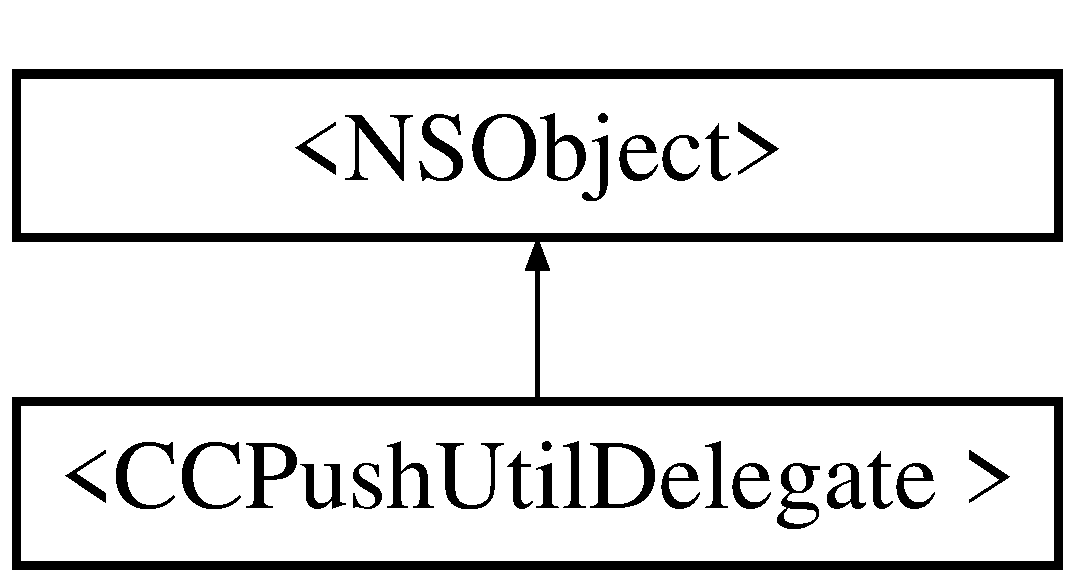
\includegraphics[height=2.000000cm]{protocol_c_c_push_util_delegate_01-p}
\end{center}
\end{figure}
\subsection*{构造函数}
\begin{DoxyCompactItemize}
\item 
\mbox{\Hypertarget{protocol_c_c_push_util_delegate_01-p_a801c02b63ee0bb894529aaf2b947a697}\label{protocol_c_c_push_util_delegate_01-p_a801c02b63ee0bb894529aaf2b947a697}} 
(void) -\/ \hyperlink{protocol_c_c_push_util_delegate_01-p_a801c02b63ee0bb894529aaf2b947a697}{room\+Name\+:}
\begin{DoxyCompactList}\small\item\em room\+Name登录成功时,会有回调返回房间名称 \end{DoxyCompactList}\item 
\mbox{\Hypertarget{protocol_c_c_push_util_delegate_01-p_a3b3b62ec6d1afd33c29fcec6d36b2560}\label{protocol_c_c_push_util_delegate_01-p_a3b3b62ec6d1afd33c29fcec6d36b2560}} 
(void) -\/ \hyperlink{protocol_c_c_push_util_delegate_01-p_a3b3b62ec6d1afd33c29fcec6d36b2560}{request\+Login\+Succeed\+With\+Viewer\+Id\+:}
\begin{DoxyCompactList}\small\item\em 登录请求成功 \end{DoxyCompactList}\item 
\mbox{\Hypertarget{protocol_c_c_push_util_delegate_01-p_abe40a1801f00e0c23b772a9c5f67dbce}\label{protocol_c_c_push_util_delegate_01-p_abe40a1801f00e0c23b772a9c5f67dbce}} 
(void) -\/ \hyperlink{protocol_c_c_push_util_delegate_01-p_abe40a1801f00e0c23b772a9c5f67dbce}{request\+Login\+Failed\+:reason\+:}
\begin{DoxyCompactList}\small\item\em 登录请求失败 \end{DoxyCompactList}\item 
\mbox{\Hypertarget{protocol_c_c_push_util_delegate_01-p_aa5f407ffe96a448cb03c7c1f534f1b0f}\label{protocol_c_c_push_util_delegate_01-p_aa5f407ffe96a448cb03c7c1f534f1b0f}} 
(void) -\/ \hyperlink{protocol_c_c_push_util_delegate_01-p_aa5f407ffe96a448cb03c7c1f534f1b0f}{push\+Failed\+:reason\+:}
\begin{DoxyCompactList}\small\item\em 推流失败 \end{DoxyCompactList}\item 
\mbox{\Hypertarget{protocol_c_c_push_util_delegate_01-p_a90d9ba4687cbdbca67be786ebbecda25}\label{protocol_c_c_push_util_delegate_01-p_a90d9ba4687cbdbca67be786ebbecda25}} 
(void) -\/ \hyperlink{protocol_c_c_push_util_delegate_01-p_a90d9ba4687cbdbca67be786ebbecda25}{is\+Connection\+Net\+Work}
\begin{DoxyCompactList}\small\item\em 正在连接网络,注:可以进行一些\+U\+I的操作 \end{DoxyCompactList}\item 
\mbox{\Hypertarget{protocol_c_c_push_util_delegate_01-p_aa8a35146fddf6ac746301d833c378a14}\label{protocol_c_c_push_util_delegate_01-p_aa8a35146fddf6ac746301d833c378a14}} 
(void) -\/ \hyperlink{protocol_c_c_push_util_delegate_01-p_aa8a35146fddf6ac746301d833c378a14}{connected\+Net\+Work\+Finished}
\begin{DoxyCompactList}\small\item\em 连接网络完成 \end{DoxyCompactList}\item 
\mbox{\Hypertarget{protocol_c_c_push_util_delegate_01-p_a8a375a1f842047cb5bc1ec497bd76992}\label{protocol_c_c_push_util_delegate_01-p_a8a375a1f842047cb5bc1ec497bd76992}} 
(void) -\/ \hyperlink{protocol_c_c_push_util_delegate_01-p_a8a375a1f842047cb5bc1ec497bd76992}{set\+Connection\+Status\+:}
\begin{DoxyCompactList}\small\item\em 设置连接状态 status含义 1\+:正在连接,3\+:已连接(表示推流成功),5\+:未连接(表示推流失败) \end{DoxyCompactList}\item 
\mbox{\Hypertarget{protocol_c_c_push_util_delegate_01-p_a4f912a0a5ef8a60d5a10f10792b83a91}\label{protocol_c_c_push_util_delegate_01-p_a4f912a0a5ef8a60d5a10f10792b83a91}} 
(void) -\/ \hyperlink{protocol_c_c_push_util_delegate_01-p_a4f912a0a5ef8a60d5a10f10792b83a91}{get\+Liveid\+Befor\+Push\+:}
\begin{DoxyCompactList}\small\item\em 点击开始推流按钮,获取liveid \end{DoxyCompactList}\item 
\mbox{\Hypertarget{protocol_c_c_push_util_delegate_01-p_a21bdf78f6576a1c1160a3a84c3ddb414}\label{protocol_c_c_push_util_delegate_01-p_a21bdf78f6576a1c1160a3a84c3ddb414}} 
(void) -\/ \hyperlink{protocol_c_c_push_util_delegate_01-p_a21bdf78f6576a1c1160a3a84c3ddb414}{node\+List\+Dic\+:best\+Node\+Index\+:}
\begin{DoxyCompactList}\small\item\em 说明:在登录时会自动进行一次测速,测速结果通过以下代理通知给用户: 返回节点列表,节点测速时间,以及最优点索引 (从0开始,如果无最优点,随机获取节点当作最优节点) 注1:字典中key为节点名称:value为一个字典,字典中有key\+:"time\char`\"{}表示测速时间(ms)和key\+:@\char`\"{}index"表示节点索引 注2:筛选的节点有一个名称为全球节点,当其他节点推流困难或推不上流时,可用这个全球节点推流,全球节点不进行测速, 故没有测速结果 \end{DoxyCompactList}\item 
\mbox{\Hypertarget{protocol_c_c_push_util_delegate_01-p_a08b40a10250ad192aa54dc7ce80d100e}\label{protocol_c_c_push_util_delegate_01-p_a08b40a10250ad192aa54dc7ce80d100e}} 
(void) -\/ \hyperlink{protocol_c_c_push_util_delegate_01-p_a08b40a10250ad192aa54dc7ce80d100e}{on\+\_\+private\+\_\+chat\+:}
\begin{DoxyCompactList}\small\item\em 收到私聊信息 \end{DoxyCompactList}\item 
\mbox{\Hypertarget{protocol_c_c_push_util_delegate_01-p_aec14126f4a940b90241b417dd142c5ca}\label{protocol_c_c_push_util_delegate_01-p_aec14126f4a940b90241b417dd142c5ca}} 
(void) -\/ \hyperlink{protocol_c_c_push_util_delegate_01-p_aec14126f4a940b90241b417dd142c5ca}{on\+\_\+chat\+\_\+message\+:}
\begin{DoxyCompactList}\small\item\em 收到公聊信息 \end{DoxyCompactList}\item 
\mbox{\Hypertarget{protocol_c_c_push_util_delegate_01-p_a70508a1bbd73495584a45887d6871c6b}\label{protocol_c_c_push_util_delegate_01-p_a70508a1bbd73495584a45887d6871c6b}} 
(void) -\/ \hyperlink{protocol_c_c_push_util_delegate_01-p_a70508a1bbd73495584a45887d6871c6b}{room\+\_\+user\+\_\+count\+:}
\begin{DoxyCompactList}\small\item\em 获取当前在线人数 \end{DoxyCompactList}\item 
\mbox{\Hypertarget{protocol_c_c_push_util_delegate_01-p_acc3ef3eb53eef99e8271da1d44bb5d3b}\label{protocol_c_c_push_util_delegate_01-p_acc3ef3eb53eef99e8271da1d44bb5d3b}} 
(void) -\/ \hyperlink{protocol_c_c_push_util_delegate_01-p_acc3ef3eb53eef99e8271da1d44bb5d3b}{receive\+Publisher\+Id\+:online\+Users\+:}
\begin{DoxyCompactList}\small\item\em 获取房间用户列表 \end{DoxyCompactList}\item 
\mbox{\Hypertarget{protocol_c_c_push_util_delegate_01-p_af64a29602fad3c4385c59a4db2d9f5b3}\label{protocol_c_c_push_util_delegate_01-p_af64a29602fad3c4385c59a4db2d9f5b3}} 
(void) -\/ \hyperlink{protocol_c_c_push_util_delegate_01-p_af64a29602fad3c4385c59a4db2d9f5b3}{stop\+Push\+Successful}
\begin{DoxyCompactList}\small\item\em 停止推流成功 \end{DoxyCompactList}\item 
\mbox{\Hypertarget{protocol_c_c_push_util_delegate_01-p_ab73312f335d91ce6341ebedefead819d}\label{protocol_c_c_push_util_delegate_01-p_ab73312f335d91ce6341ebedefead819d}} 
(void) -\/ \hyperlink{protocol_c_c_push_util_delegate_01-p_ab73312f335d91ce6341ebedefead819d}{custom\+Message\+:}
\begin{DoxyCompactList}\small\item\em 用户自定义消息 \end{DoxyCompactList}\end{DoxyCompactItemize}


该协议的文档由以下文件生成\+:\begin{DoxyCompactItemize}
\item 
C\+C\+Push\+Util.\+h\end{DoxyCompactItemize}

\hypertarget{interface_push_parameters}{}\section{Push\+Parameters类 参考}
\label{interface_push_parameters}\index{Push\+Parameters@{Push\+Parameters}}
类 Push\+Parameters 继承关系图\+:\begin{figure}[H]
\begin{center}
\leavevmode
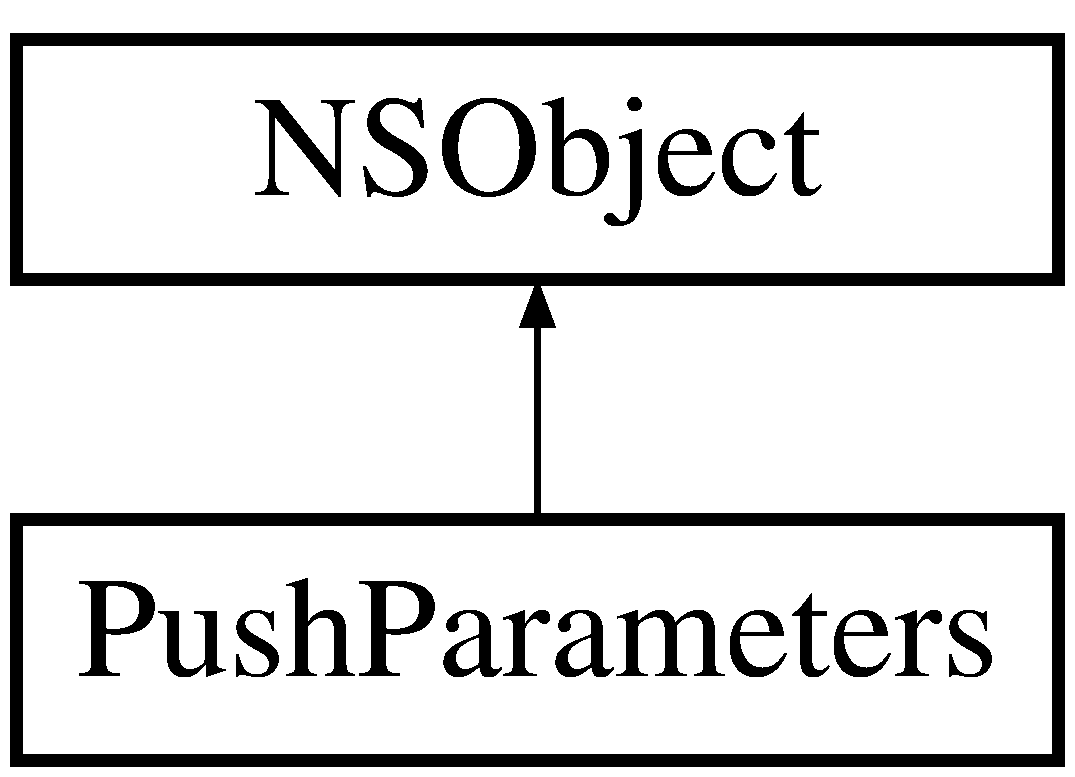
\includegraphics[height=2.000000cm]{interface_push_parameters}
\end{center}
\end{figure}
\subsection*{属性}
\begin{DoxyCompactItemize}
\item 
\mbox{\Hypertarget{interface_push_parameters_a722b1e94179f3d816ef369d29bf28fe6}\label{interface_push_parameters_a722b1e94179f3d816ef369d29bf28fe6}} 
N\+S\+String $\ast$ \hyperlink{interface_push_parameters_a722b1e94179f3d816ef369d29bf28fe6}{user\+Id}
\begin{DoxyCompactList}\small\item\em 用户\+ID \end{DoxyCompactList}\item 
\mbox{\Hypertarget{interface_push_parameters_a33af8d25a2f144afca8e77ffb9e31082}\label{interface_push_parameters_a33af8d25a2f144afca8e77ffb9e31082}} 
N\+S\+String $\ast$ \hyperlink{interface_push_parameters_a33af8d25a2f144afca8e77ffb9e31082}{room\+Id}
\begin{DoxyCompactList}\small\item\em 直播间号 \end{DoxyCompactList}\item 
\mbox{\Hypertarget{interface_push_parameters_a1d607c97abf94d67a0e413df87422a2d}\label{interface_push_parameters_a1d607c97abf94d67a0e413df87422a2d}} 
N\+S\+String $\ast$ \hyperlink{interface_push_parameters_a1d607c97abf94d67a0e413df87422a2d}{viewer\+Name}
\begin{DoxyCompactList}\small\item\em 用户名称 \end{DoxyCompactList}\item 
\mbox{\Hypertarget{interface_push_parameters_a4a6e4b2ad16ee88c4555a8541d085864}\label{interface_push_parameters_a4a6e4b2ad16ee88c4555a8541d085864}} 
N\+S\+String $\ast$ \hyperlink{interface_push_parameters_a4a6e4b2ad16ee88c4555a8541d085864}{token}
\begin{DoxyCompactList}\small\item\em 密码 \end{DoxyCompactList}\item 
\mbox{\Hypertarget{interface_push_parameters_ab12c8665dcbc45b0c369a21b3992a191}\label{interface_push_parameters_ab12c8665dcbc45b0c369a21b3992a191}} 
B\+O\+OL \hyperlink{interface_push_parameters_ab12c8665dcbc45b0c369a21b3992a191}{security}
\begin{DoxyCompactList}\small\item\em 是否使用https,\+Y\+ES\+:https NO\+:http \end{DoxyCompactList}\end{DoxyCompactItemize}


该类的文档由以下文件生成\+:\begin{DoxyCompactItemize}
\item 
Push\+Parameters.\+h\end{DoxyCompactItemize}

%--- End generated contents ---

% Index
\backmatter
\newpage
\phantomsection
\clearemptydoublepage
\addcontentsline{toc}{chapter}{索引}
\printindex

\end{document}
